\documentclass[11pt,letterpaper]{article}

\usepackage[top=1in,bottom=1in,left=1.15in,right=1.15in]{geometry}
\usepackage{lmodern}
\PassOptionsToPackage{hyphens}{url}
\usepackage{hyperref}
\usepackage{url}
\usepackage{booktabs}
\usepackage{array}
\usepackage{graphicx}
\usepackage{float}
\usepackage{titlesec}
\usepackage{enumitem}
\usepackage{fancyhdr}
\usepackage{xcolor}

% Section styling
\titleformat{\section}{\large\bfseries}{}{0em}{}[\titlerule]
\titlespacing{\section}{0pt}{1.4em}{0.5em}
\titleformat{\subsection}{\normalsize\bfseries}{}{0em}{}
\titlespacing{\subsection}{0pt}{0.9em}{0.3em}

% Body spacing
\setlength{\parskip}{0.5em}
\setlength{\parindent}{0pt}
\setlist{noitemsep, topsep=0.3em}

% Links
\hypersetup{colorlinks=true, urlcolor=blue!70!black, linkcolor=black, breaklinks=true}
\urlstyle{same}
\def\UrlBreaks{\do\/\do-\do\_\do\#\do.}
\setlength{\emergencystretch}{4em}

% Header / footer
\pagestyle{fancy}
\fancyhf{}
\renewcommand{\headrulewidth}{0.4pt}
\lhead{\small UBBX — UB Book Exchange}
\rhead{\small CSE 426 Term Project}
\cfoot{\small\thepage}

\begin{document}

% ── Title block ────────────────────────────────────────────────────────────────
\begin{center}
  {\LARGE\bfseries UBBX (UB Book Exchange)}\\[0.4em]
  {\large CSE 426 Term Project Documentation}\\[0.3em]
  {\normalsize Puru Soni \quad|\quad May 2, 2026}
\end{center}

\vspace{0.4em}
\noindent
\begin{tabular}{@{} >{\bfseries}p{0.20\linewidth}
                    >{\raggedright\arraybackslash}p{0.76\linewidth} @{}}
Live Project   & \url{https://ubbx.purusoni.com} \\
Repository     & \url{https://github.com/purusoni/UBBX} \\
UBBX Contract  & \texttt{0x780ef830cc76AD6E88FCe62A0e0485b68c227C41} \\
Yoda Token     & \texttt{0xbd27d0b7F9fedb5A2A2C3ceF5dC9c70f3CF64Af2} \\
\end{tabular}

% ── 1 ─────────────────────────────────────────────────────────────────────────
\section{Project Overview}

UBBX is a decentralized textbook marketplace on Ethereum Sepolia.
Listings are priced in Yoda (ERC-20) and participants transact directly through
a wallet-connected web interface.

\subsection*{Motivation}

University students frequently accumulate course textbooks that have little value
to them after completing a class, while students entering those same courses face
high retail and buyback prices. UBBX connects these two groups peer-to-peer,
using a smart contract as the neutral intermediary for payment settlement and
record-keeping.

% ── 2 ─────────────────────────────────────────────────────────────────────────
\section{Design Details}

\subsection*{Smart Contract}

The core marketplace logic is in \texttt{contracts/UBBX.sol}.

\begin{itemize}
  \item \texttt{listBook(isbn, priceYoda, condition, metadataHash)} registers a
        listing and emits \texttt{BookListed}.
  \item \texttt{purchaseBook(id)} transfers Yoda from buyer to seller via
        \texttt{transferFrom}, marks the listing sold, and emits
        \texttt{BookPurchased}.
\end{itemize}

\subsection*{Data Design}

On-chain state stores the minimum needed for trustless settlement: ISBN, price,
condition, availability, and seller address. Descriptive content (title, author,
edition, notes, image, contact) is stored off-chain in
\texttt{metadata/<listingId>.json}. An optional \texttt{metadataHash} field
allows buyers to verify catalog integrity on-chain.

\subsection*{Front End}

The web interface is a static site served from the repository root
(\texttt{index.html}, \texttt{app.js}), integrated with MetaMask and ethers.js v5.
Listings are browsable without a wallet connection; listing and purchasing require
one.

% ── 3 ─────────────────────────────────────────────────────────────────────────
\section{Development Details}

\begin{center}
\begin{tabular}{@{} >{\bfseries}l l @{}}
\toprule
Component    & Files \\
\midrule
Contract     & \texttt{contracts/UBBX.sol} \\
Front end    & \texttt{index.html},\ \texttt{app.js} \\
ABIs         & \texttt{UBBX.json},\ \texttt{yoda.json} \\
Metadata     & \texttt{metadata/*.json} \\
\bottomrule
\end{tabular}
\end{center}

Verified Sepolia transactions:

\begin{center}
\begin{tabular}{@{} >{\bfseries}l l r @{}}
\toprule
Type & Truncated hash & Fee (ETH) \\
\midrule
Deploy        & \texttt{0x3cd90f7473cbc6...} & 0.001623567 \\
List Book     & \texttt{0x4e8d3b2e7bb379...} & 0.000243504 \\
Purchase Book & \texttt{0x8783668c41563f...} & 0.000108770 \\
List Book     & \texttt{0xc74592d99d8189...} & 0.000222612 \\
Purchase Book & \texttt{0x17b01343ffe345...} & 0.000083120 \\
List Book     & \texttt{0x9214c5506645c1...} & 0.000222612 \\
\bottomrule
\end{tabular}
\end{center}

% ── 4 ─────────────────────────────────────────────────────────────────────────
\section{How to Run the Code}

\subsection*{Local Test}

Serve the repository root over HTTP and open it in a browser:

\begin{verbatim}
python3 -m http.server 8080
\end{verbatim}

Connect MetaMask and switch to Sepolia.

\subsection*{Deployment}

\begin{enumerate}
  \item Compile and deploy \texttt{contracts/UBBX.sol} (Solidity \texttt{\^{}0.8.28})
        with the Yoda token address as the constructor argument.
  \item Set \texttt{ubbxAddress} and \texttt{yodaAddress} in \texttt{app.js}.
  \item Publish the static site via GitHub Pages (branch: \texttt{main}, folder: root).
  \item For each listing with a metadata hash, commit the corresponding
        \texttt{metadata/<id>.json} file and push.
\end{enumerate}

\begin{figure}[H]
  \centering
  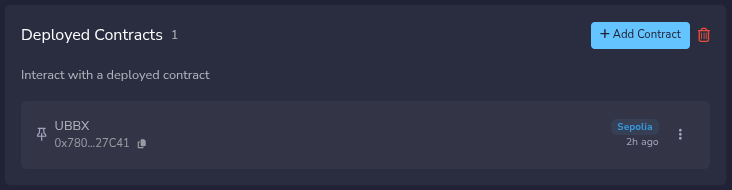
\includegraphics[width=0.72\linewidth]{remix-deployed.png}
  \caption{Remix IDE showing UBBX contract deployed at
           \texttt{0x780\ldots 27C41} on Sepolia.}
\end{figure}

\begin{figure}[H]
  \centering
  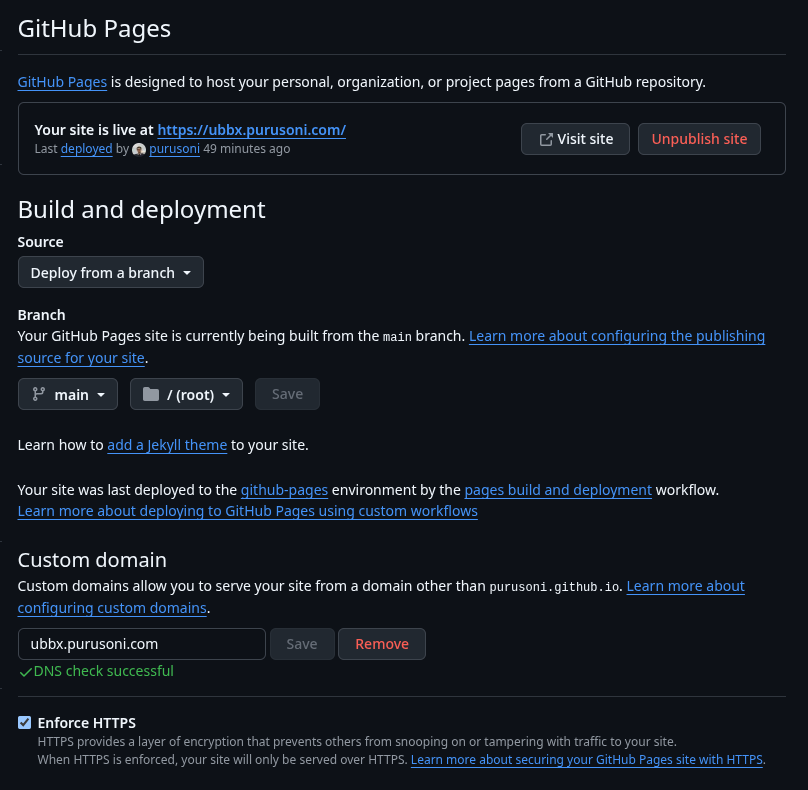
\includegraphics[width=0.9\linewidth]{github-pages-settings.png}
  \caption{GitHub Pages configuration: \texttt{main} branch, root folder, custom
           domain \texttt{ubbx.purusoni.com}, HTTPS enforced.}
\end{figure}

% ── 5 ─────────────────────────────────────────────────────────────────────────
\section{User Instructions}

\begin{enumerate}
  \item Open \url{https://ubbx.purusoni.com} and connect MetaMask on Sepolia.
  \item To list a book: enter ISBN, Yoda price, condition, and optional metadata
        fields, then submit.
  \item To buy: select a listing from the catalog, enter its ID in the buy panel,
        approve Yoda spending if prompted, then confirm the purchase.
  \item Transaction confirmation and listing status updates appear in the UI.
\end{enumerate}

\noindent Wallets used in testing:
\begin{itemize}
  \item Seller: \texttt{0xC6E031b6bd83891efFe6bAA15d7F7Df11549E9e1}
  \item Buyer:  \texttt{0x59Fb57c7D932d1a61915df7C095Def91627567fa}
\end{itemize}

\begin{figure}[H]
  \centering
  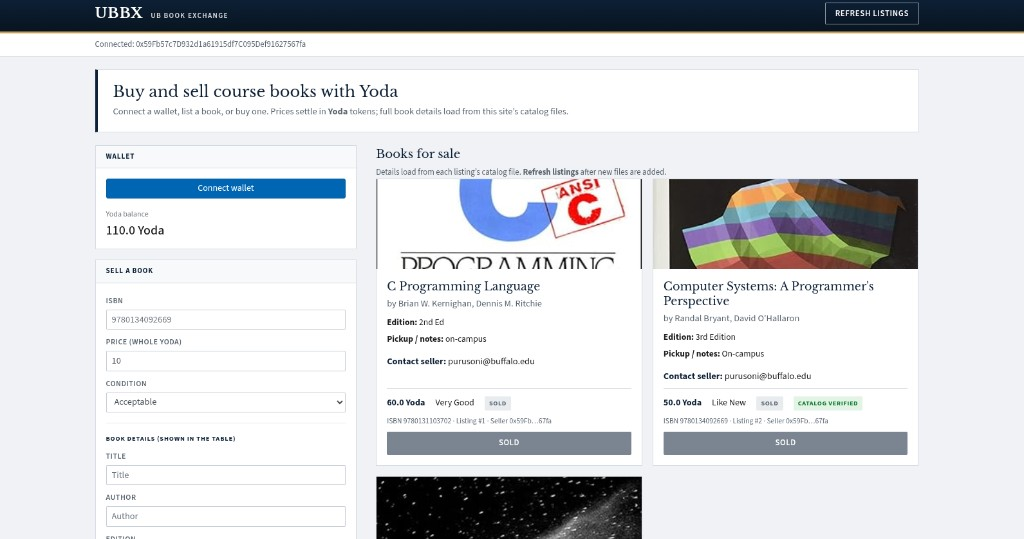
\includegraphics[width=\linewidth]{ui-full-page.png}
  \caption{UBBX marketplace showing listed books, Yoda balance, and sell form.}
\end{figure}

\begin{figure}[H]
  \centering
  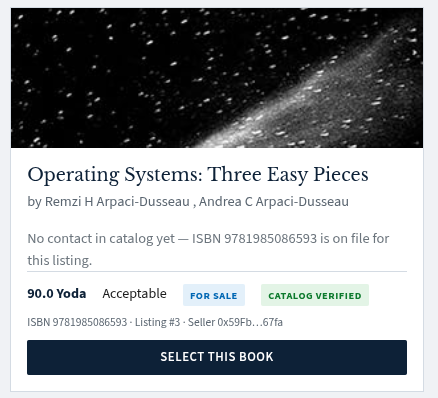
\includegraphics[width=0.65\linewidth]{ui-listing-card.png}
  \caption{Individual listing card: price, condition, and catalog verification badge.}
\end{figure}

\begin{figure}[H]
  \centering
  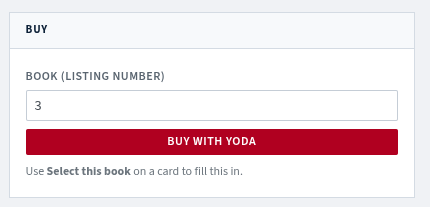
\includegraphics[width=0.6\linewidth]{ui-buy-panel.png}
  \caption{Buy panel with listing ID pre-filled from catalog selection.}
\end{figure}

% ── 6 ─────────────────────────────────────────────────────────────────────────
\section{Performance Metrics}

\begin{center}
\begin{tabular}{@{} >{\bfseries}p{0.42\linewidth} p{0.50\linewidth} @{}}
\toprule
Metric & Value \\
\midrule
Total contract transactions   & 6 (1 deploy, 3 list, 2 purchase) \\
ERC-20 token transfer events  & 3 \\
Avg.\ fee (non-deploy, 5 tx)  & 0.000176 ETH \\
\bottomrule
\end{tabular}
\end{center}

Data sources:
\begin{itemize}
  \item \url{https://sepolia.etherscan.io/address/0x780ef830cc76AD6E88FCe62A0e0485b68c227C41}
  \item \url{https://sepolia.etherscan.io/address/0xC6E031b6bd83891efFe6bAA15d7F7Df11549E9e1#tokentxns}
  \item \url{https://sepolia.etherscan.io/address/0x59Fb57c7D932d1a61915df7C095Def91627567fa#tokentxns}
\end{itemize}

\begin{figure}[H]
  \centering
  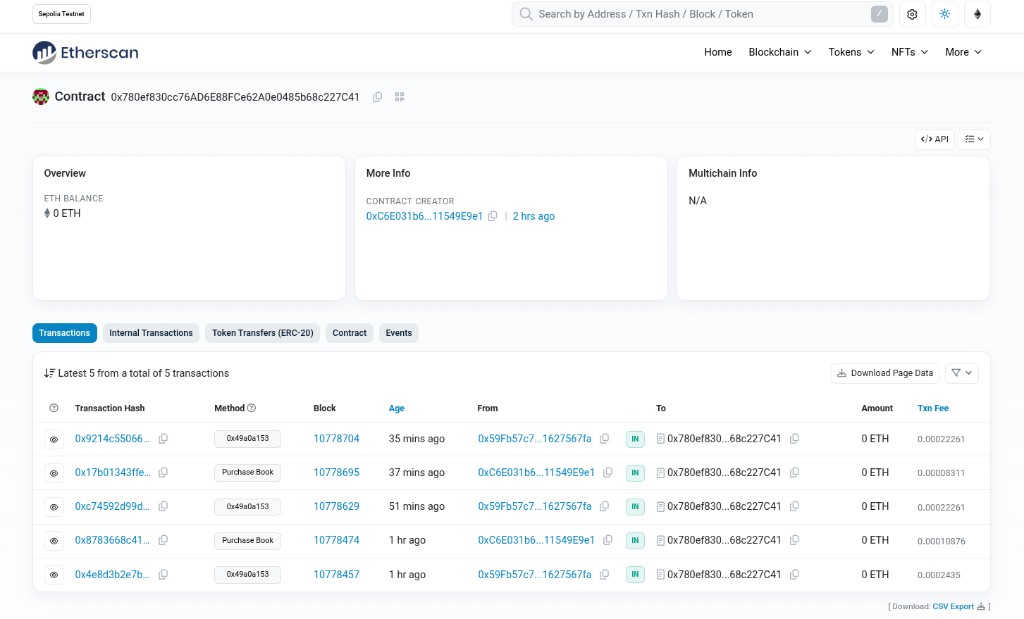
\includegraphics[width=\linewidth]{etherscan-contract-transactions.png}
  \caption{Contract transaction history on Sepolia with gas fees.}
\end{figure}

\begin{figure}[H]
  \centering
  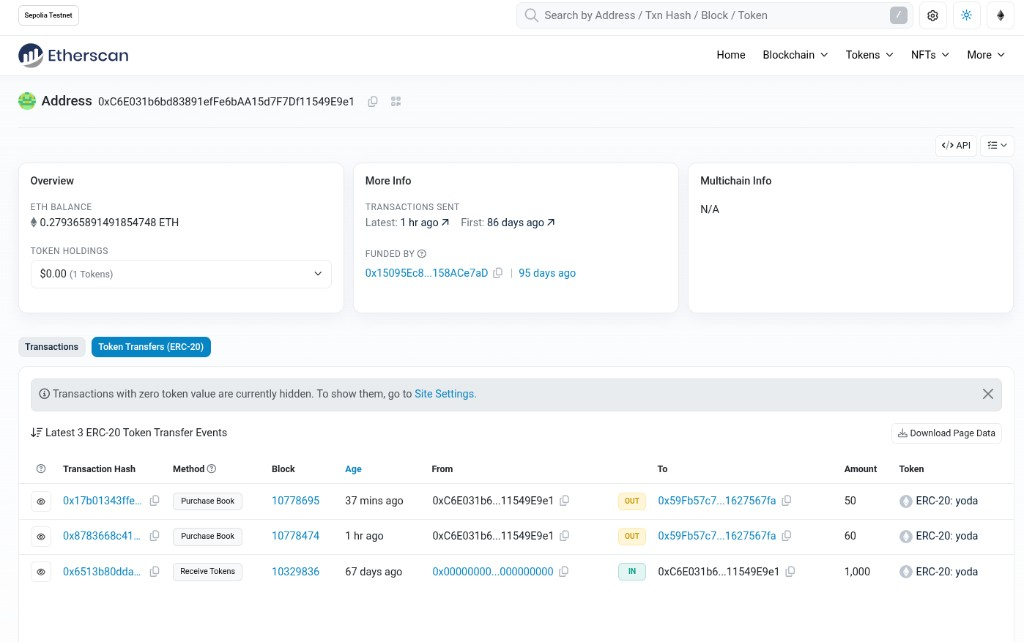
\includegraphics[width=\linewidth]{etherscan-token-transfers.png}
  \caption{Yoda ERC-20 token transfers from the seller wallet.}
\end{figure}

\begin{figure}[H]
  \centering
  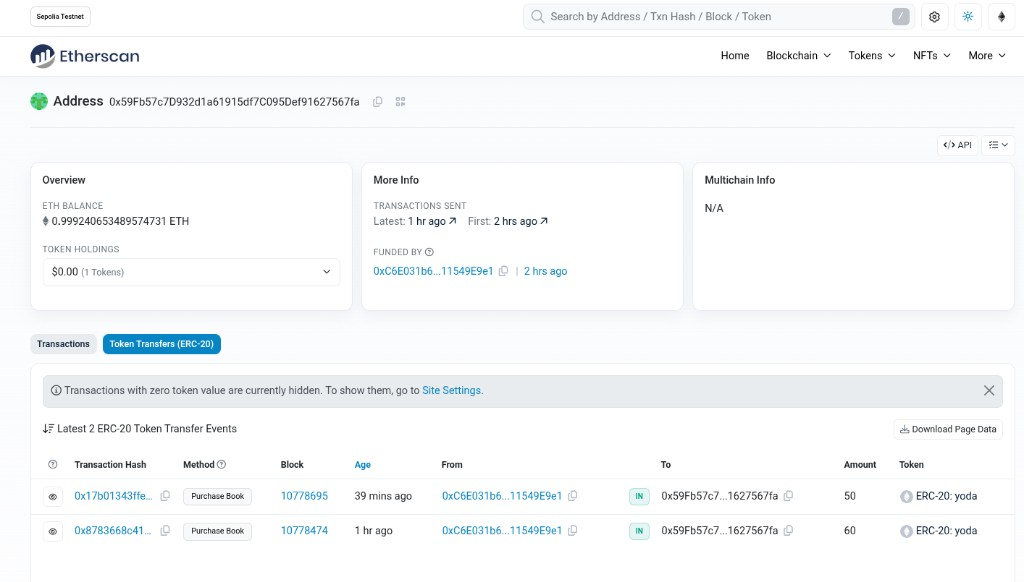
\includegraphics[width=\linewidth]{etherscan-token-transfers-account2.png}
  \caption{Yoda ERC-20 token transfers received by the buyer wallet.}
\end{figure}

% ── AI note ───────────────────────────────────────────────────────────────────
\section{Use of AI Tools}

Cursor (an AI-assisted IDE) was used as a development aid for code refactoring
and documentation drafting. Project architecture, contract design, deployment,
and testing were directed by the student.

\end{document}
